\chapter{Case Study: Collaborative Knowledge-Management Platform}

In this chapter, we will discuss an example application of the collaborative modeling framework in detail. Using the framework, I modeled a collaborative knowledge-management platform. This application allows a group of people to create sessions and collaborate on a research project. Most of the components and collaborative patterns incorporated into the framework have been used in order to model this case study application. 

\section{Collaborative Knowledge-Management Platform}

The goal of this case study is to show the capabilities of the collaborative modeling framework. I modeled an application, using the framework, that proposes a prototype that should make it easier for researchers to collaborate on research projects.

\subsection{Problem}

Currently, there is no collaborative Android application that allows people to work on a research project. This prototype proposal should help researchers on communicating and collaborating through Android phones. For instance, when reading papers, a researcher typically wants to make notes on them. It should be possible to create and share notes easily with a research group. Currently, people make notes in the margin of a paper and pass this paper on to other people. This method does not encourage collaboration and it's hard to collaborate in real-time when both people want to read the same paper. Moreover, this classical approach is not scalable to a group of researchers. \\ \\
A second problem goes back to collaboration in real-time. When two researchers are not in the same place (and/or time), it is hard to collaborate in real-time on a research project. How do people working on a research project keep in sync at all the times? We currently have access to the technology, we only need to build the right tools with this technology. If we use technology as an enabler to work more efficiently (i.e. create the tools), how will this make us more efficient on a research project?

\subsection{Solution}

It looks like the solution to the problem that I analyzed is twofold:
\begin{itemize}
\item{In order to solve the first problem, we can introduce an annotation layer on top of a repository. In the collaborative modeling framework, a repository is modeled using a Dropbox folder. The metadata of every item in this folder can be fetched and annotated with a note by one of the registered researchers of the application. This allows people to simultaneously share their insights on new papers.} 
\item{When we want to allow a group of researchers to truly collaborate in real-time when they are not in the same place, we have to introduce a way to make it possible to easily communicate with current technology constraints. This problem is solved by integrating a chat box that allows a team to have a discussion in real-time, whether they are in the same place at the same time or not.}
\end{itemize}
In addition to solutions to those problems, the case study also includes other mechanisms that create awareness between researchers and helps them identify their research goals. In the following section, implementation details of these needs and features will be discussed.

\section{Platform implementation}

The main entities of the model for the Collaborative Knowledge-Management Platform are the Android activities. These activities represent the main features found in the application. Each of those are embedded in a main \texttt{Application} object. All source code can be found on Github\footnote{https://github.com/philipdesmedt/Thesis-Android} \cite{Github}. We will discuss the most important activities in depth in this section\footnote{Note that all references not explained in the meta-models, are simply references to other Metadepth meta-models in the collaborative modeling framework}:
\begin{itemize}
\item{LoginActivity}
\item{MainActivity}
\item{ListActivity}
\end{itemize} 

\subsection{LoginActivity}

The model for \texttt{LoginActivity} is listed as follows:

\begin{lstlisting}[label=login-model,caption=LoginActivity model, captionpos=t]
Activity act1 {
	name = "LoginActivity";
	main = true;

	content = [login];
	presentation = pres1;
}
\end{lstlisting}
Following the \texttt{Activity} meta-model, we have set the \texttt{LoginActivity} model to be the main \texttt{Activity} (which means it will be the first one to be started by the Android OS). As a component, we include a login component and set the layout (which contains two textfields to authenticate, one for the username and for the password, and a button to initiate the login action). The login component is defined as follows:

\begin{lstlisting}[label=logincomponent-model,caption=Login component model, captionpos=t]
Login login {
	host = "10.0.2.2";
	port = "3000";

	layoutcomponents = [usernameView, usernameText, passwordView, passwordText, loginButton];
	actions = [ela1, ela2];
	uiactions = [triggerLogin];
}
\end{lstlisting}
Both the \texttt{host} and \texttt{port} fields are settings that should be set to connect to the server users should authenticate with. The layout components are, as mentioned earlier, the inputs for authentication with the server. The \texttt{actions} list  extends the functionality of the \texttt{action} method of a component and the \texttt{uiactions} list contains actions that will be executed on UI elements in the application. In the login component, \texttt{ela1} and \texttt{ela2} are both \texttt{ExtractLayoutAction} elements that extract both the username and the password from UI elements and use these in the \texttt{action} method to pass credentials to the server. The UI action \texttt{triggerLogin} specifies what has to be done when the login button is triggered. This specific action effectively calls the \texttt{action} method of our login component and changes the Activity to \texttt{MainActivity} when the given credentials are verified. If the credentials are incorrect, nothing happens at all.

\subsection{MainActivity}

The \texttt{MainActivity} class is the entry point for our application once the user is logged in successfully. It contains shortcuts to all functionality within the app. This activity is modeled as follows:

\begin{lstlisting}[label=main-model,caption=MainActivity model, captionpos=t]
MainActivity act2 {
	name = "MainActivity";
	main = false;

	content = [twitter];
	presentation = pres2;
	onClickListeners = [triggerChat, triggerDropbox, triggerGoals, triggerLogout];
	userView = connectedUsers;
}
\end{lstlisting}
We only modeled one component in \texttt{MainActivity}, a Twitter component. We don't want a separate Activity for a Twitter component, so that's why we just embedded it into the current Activity and used a \texttt{Button} as a trigger for it. Because this component does not need a lot of customizations (apart from the text to tweet), it is offered as an integrated component solution in the framework. The \texttt{onClickListeners} specify all shortcuts to the other Activities in the current Activity. Finally, we also specified a \texttt{userView} field that, if set, shows all currently connected users in the application. \\ \\
Note that we don't just use the \texttt{Activity} meta-model, but the \texttt{MainActivity} meta-model. This meta-model has no difference with the \texttt{Activity} meta-model on a modeling level, but it has some differences on the implementation level. The \texttt{MainActivity.java} implementation inherits from the \texttt{Activity} implementation included in the Android SDK. It is an \texttt{abstract class} that requires  the implementation of the \texttt{setConnectedUsers} method. This method takes a \texttt{String} of users as input and allows a modeler to show the currently connected users. That way, our collaborative framework can easily support the awareness of users in a collaborative application.

\subsection{ListActivity}

Another important Activity is the model of the \texttt{ListActivity}. We use this generic Activity to allow the implementation of lists of various forms in our application. This way we could model the annotation of Dropbox notes, a list of goals or a questionnaire that can have an arbitrary number of answers. The model for this generic activity is listed in listing ~\ref{list-model}.
\begin{lstlisting}[label=list-model,caption=ListActivity model, captionpos=t]
GenericActivity act5 {
	name = "ListActivity";
	main = false;

	content = [list];
	presentation = pres5;
}
\end{lstlisting}
The most important aspect of this model is the use of the \texttt{GenericActivity} meta-model type. Just like the \texttt{MainActivity} meta-model, this meta-model has no difference with the \texttt{Activity} meta-model, but the implementation again is slightly different. \texttt{GenericActivity} is an abstract class that contains two abstract methods, \texttt{AndroidComponent getComponent()} and \texttt{void onMessage(String user, String message)}. The \texttt{getComponent()} method is used when we need to notify the embedded component within this Activity and the \texttt{onMessage()} method is a callback function that is called when we receive a message from the server. Usually, those \texttt{GenericActivity} classes also have a child Activity associated with them, in particular when we implement a list component. This child activity is used to display the comments or notes on a particular list item. For instance, if we model a list of goals, we can comment on these goals. These comments are wrapped into the child activity.

\section{Demonstration}

In this section, we will have a look at the running modeled application. In the previous section, the several activities and their models were discussed and now we can see them in action. In figure ~\ref{fig:coll_connected}, we see the main activity after a user successfully logged in. In this activity, a user can navigate to all other activities in the collaborative application.
\begin{figure}[h!]
\centering
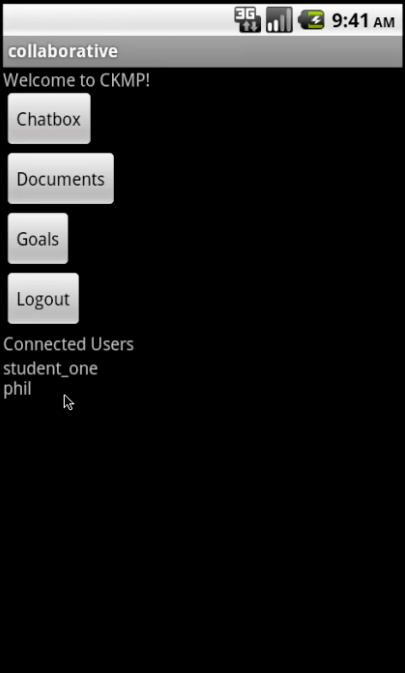
\includegraphics[width=0.4\textwidth]{images/chap7_connected.png}
\caption{In the main menu of the collaborative application with two connected users}
\label{fig:coll_connected}
\end{figure} \\ \\
When we start the chat activity, a simple screen with the latest chat messages comes up. A user can then send a message to all other users. This message will be persisted in a MongoDB database and subsequently be sent to all users. A view of the chat box is depicted in figure ~\ref{fig:coll_chatbox}. 
\begin{figure}[h!]
\centering
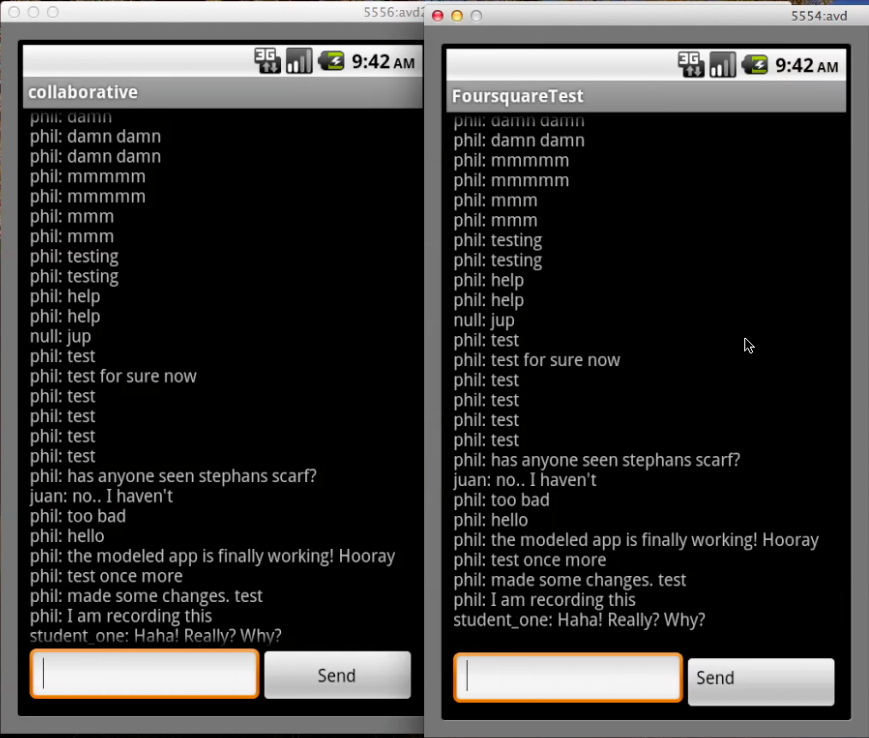
\includegraphics[width=0.99\textwidth]{images/chap7_chatbox.png}
\caption{In the chat box of the collaborative application}
\label{fig:coll_chatbox}
\end{figure} \\ \\
Finally, the functionality of the Dropbox repository is depicted in figures ~\ref{fig:coll_dropbox1} and ~\ref{fig:coll_dropbox2}. The first figure shows the content of the folder we passed when modeling the Dropbox repository. This directory contains all research papers used to write this thesis. The other figure shows notes on a particular research paper in this directory. Users are able to comment on the paper and make additional notes to e.g. remember the summary of a paper. Users with the \texttt{admin} permission can view all notes on a file. Other users with non-admin permission can only see their own comments.
\begin{figure}[h!]
\centering
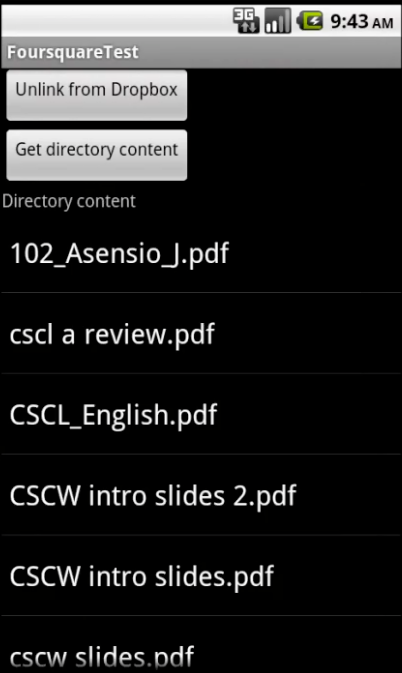
\includegraphics[width=0.4\textwidth]{images/chap7_dropbox1.png}
\caption{Fetched all research papers from the Dropbox repository}
\label{fig:coll_dropbox1}
\end{figure}
\begin{figure}[h!]
\centering
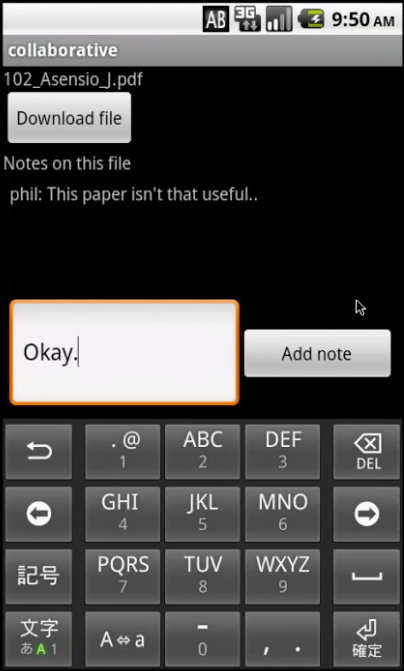
\includegraphics[width=0.4\textwidth]{images/chap7_dropbox2.png}
\caption{Notes and comments on a research paper in the Dropbox repository}
\label{fig:coll_dropbox2}
\end{figure}
